\chapter{Electromagnetic Waves}
\section{Cable Waves}
Before getting into Maxwell's equations and the wave equation for light, consider the electromagnetic waves that propagate down a coaxial cable.

To get a handle on the coaxial cable, consider the idealized circuit below
\begin{figure}[h!]
    \centering
    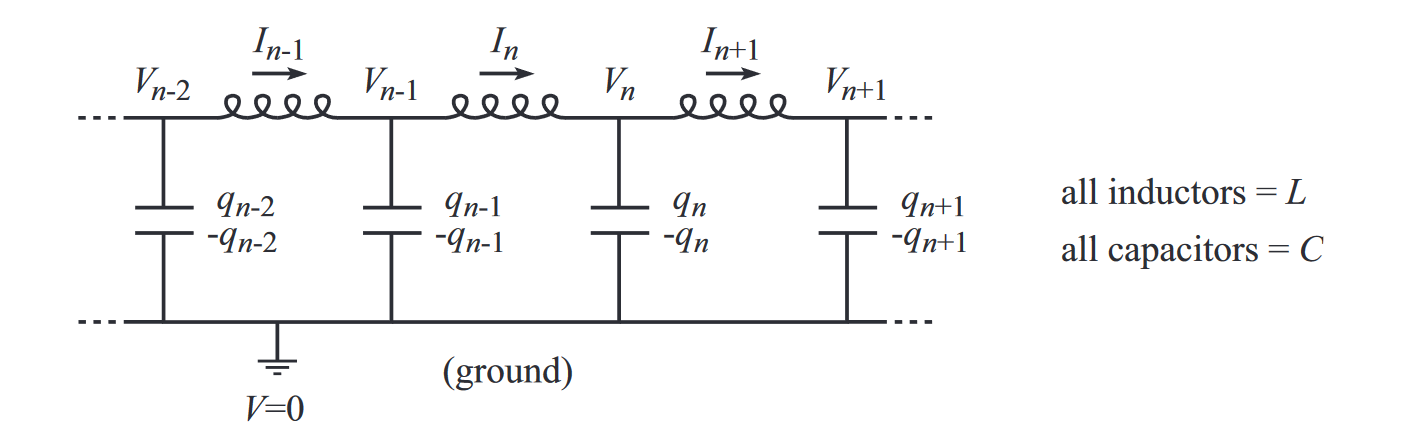
\includegraphics[width=\linewidth]{figures/circuit.png}
\end{figure}

There are three relevant facts:
\begin{enumerate}
    \item The charge on a capacitor is $Q = CV \implies q_n = CV_n$.
    \item The voltage across an inductor is $V = L(\dvi{I}{t}) \implies V_{n-1} - V_n = L(\dvi{I_n}{t})$.
    \item Conservation of charge yields $I_n - I_{n+1} = \dvi{q_n}{t}$.
\end{enumerate}
Our goal is to produce an equation for one of the three variables $q$, $I$, or $V$. This equation will turn out to be a wave equation, that is exactly the same for each variable. We could manipulate the above equations and then take the continuum limit to do this, but we will find that it is actually far easier to take the limit first and then manipulate the expressions.

If we let the width of the grid be $\Delta x$, then the above three facts become
\begin{align*}
    q &= CV \\
    -\pdv{V}{x}\Delta x &= L\pdv{I}{t} \\
    -\pdv{I}{x}\Delta x &= \pdv{q}{t}
\end{align*}
substituting $q=CV$ from the first equation into the third yields
\[ -\pdv{I}{x}\Delta x = C\pdv{V}{t} \]
Then, defining the inductance and capacitance per unit length as $L_0 \equiv L/\Delta x$ and $C_0 \equiv C/\Delta x$, we find the two equations
\[ -\pdv{V}{x} = L_0\pdv{I}{t} \quad\text{and}\quad -\pdv{I}{x} = C_0\pdv{V}{t} \]
Taking the space derivative of the first equation and the time derivative of the second, we find
\[ -\pdv[2]{V}{x} = L_0\frac{\partial ^2I}{\partial t\partial x}\quad\text{and}\quad -C_0\pdv[2]{V}{t} = \frac{\partial^2 I}{\partial x \partial t}\]
These can be set equal to each other to find
\[ \frac{1}{L_0}\pdv[2]{V}{x} = C_0\pdv[2]{V}{t}\]
or, rearranging slightly,
\[ \pdv[2]{V(x,t)}{t} = \frac{1}{L_0C_0}\pdv[2]{V(x,t)}{x} \]
this is the wave equation for a dispersionless wave with a speed
\[ c = \frac{1}{\sqrt{L_0C_0}}\]
Similar analyses show us that the exact same wave equation holds for $V$, $q$, and $I$.

Now, let's look at an actual coaxial cable. Consider a conducting wire inside a conducting cylinder, with vacuum in the region between them. Assume that the wire is somehow constrained to be in the middle of the cylinder. The cable has an inductance $L_0$ per unit length, in the same way that two parallel wires do. It also has a capacitance $C_0$ per unit length.

An arduous calculation shows that
\[ L_0 = \frac{\mu_0}{2\pi} \ln(r_2/r_1) \quad\text{and}\quad C_0 = \frac{2\pi\epsilon_0}{\ln(r_2/r_2)} \]
Thus, the wave speed is 
\[ v = \frac{1}{\sqrt{L_0C_0}} = \frac{1}{\mu_0\epsilon_0} \approx 3\times 10^8 \text{ m/s}\]
This is the speed of light! So the voltage, charge, and current waves all travel down the cable at the speed of light. And because there are electric and magnetic fields in the cable, these fields also undergo wave motion. Since the waves of these fields travel at the same speed as the original voltage wave, it is a good bet that electromagnetic waves have something to do with light. 
\section{The Wave Equation}
Maxwell's four equations govern all of electromagnetism, and here they are, in both differential and integral form:
\begin{align*}
    &\div \mbf E = \frac{\rho_E}{\epsilon_0} &&\oiint \mbf E \cdot \dd \mbf A = \frac{Q_E}{\epsilon_0} \\
    &\div \mbf B = \rho_B &&\oiint \mbf B \cdot \dd \mbf A = Q_B \\
    &\curl \mbf E = -\pdv{\mbf B}{t} + \mbf J_B &&\oint \mbf E \cdot \dd\mbf l = -\dv{\Phi_B}{t} + I_B \\
    &\curl \mbf B = \mu_0\epsilon_0 \pdv{\mbf E}{t} + \mu_0\mbf J_E &&\oint \mbf B \cdot \dd \mbf l = \mu_0\epsilon_0 \dv{\Phi_E}{t} + \mu_0 I_E
\end{align*}
If we erase the $\mu_0$'s and $\epsilon_0$'s here, which arise from the arbitrary definitions of our units, then these equations are symmetric in $\mbf E$ and $\mbf B$, save for a few minus signs. The $\rho$'s are the electric and (hypothetical) magnetic charge densities, and the $\mbf J$'s are the current densities. The $Q$'s are the charges enclosed by the surface that define the $\dd \mbf A$ integrals, and the $\Phi$'s are the field fluxes through the loops that define the $\dd\mbf l$ integrals.

No one has ever found an isolated magnetic charge, and there are various theoretical considerations that suggest they can't exist, at least in our universe. So we'll set $\rho_B$, $\mbf J_B$, and $I_B$ equal to zero from here on. This will make Maxwell's equations appear asymmetrical, but we'll soon be setting the analogous electric quantities equal to zero too. Thus, Maxwell's equations become
\begin{align*}
    &\div \mbf E = \frac{\rho_E}{\epsilon_0} &&\oiint \mbf E \cdot \dd \mbf A = \frac{Q_E}{\epsilon_0} \\
    &\div \mbf B = 0 &&\oiint \mbf B \cdot \dd \mbf A = 0 \\
    &\curl \mbf E = -\pdv{\mbf B}{t} &&\oint \mbf E \cdot \dd\mbf l = -\dv{\Phi_B}{t} \\
    &\curl \mbf B = \mu_0\epsilon_0 \pdv{\mbf E}{t} + \mu_0\mbf J_E &&\oint \mbf B \cdot \dd \mbf l = \mu_0\epsilon_0 \dv{\Phi_E}{t} + \mu_0 I_E
\end{align*}
In order, these laws are known as Gauss' Law, ``No magnetic monopoles," Faraday's law, and Ampere's law. Ampere's law includes the so-called ``displacement current" $\dvi{\Phi_E}{t}$.

Our goal is to derive the wave equation for the $\mbf E$ and $\mbf B$ fields in a vacuum. Since there are no charges in any kind of vacuum, we'll set $\rho_E$ and $\mbf J_E$ equal to zero from here on. And we'll only need the differential forms, so we now have
\begin{align*}
    \div  \mbf E &= 0 \\
    \div  \mbf B &= 0 \\
    \curl \mbf E &= -\pdv{\mbf B}{t} \\
    \curl \mbf B &= \mu_0\epsilon_0 \pdv{\mbf E}{t} 
\end{align*}
Taking the curl of the third of these equations, we find
\[ \curl(\curl \mbf E)  =-\curl \pdv{\mbf B}{t} \]
for the right side, we find
\begin{align*}
    -\curl \pdv{\mbf B}{t} &= -\pdv{t}\pqty{\curl \mbf B} \\
    &= -\pdv{t} \pqty{\mu_0\epsilon_0\pdv{\mbf E}{t}} \\
    &= -\mu_0\epsilon_0 \pdv[2]{\mbf E}{t}
\end{align*}
for the left side, we use the handy ``BAC-CAB" formula
\[ \mbf A \times (\mbf B \times \mbf C) = \mbf B(\mbf A \cdot \mbf C) - \mbf C(\mbf A\cdot \mbf B)\]
which tells us that
\begin{align*}
    \curl(\curl \mbf E) &= \grad(\div \mbf E) - \mbf E(\div \grad) \\
    &= \mbf 0 - \grad^2\mbf E = -\grad^2\mbf E
\end{align*}
Thus, we find that
\[ \boxed{\pdv[2]{\mbf E}{t} = \frac{1}{\mu_0\epsilon_0} \grad^2\mbf E} \]
We could have instead eliminated $\mbf E$ instead of $\mbf B$, which would give us exactly the same wave equation (since Maxwell's equations are symmetric),
\[ \boxed{\pdv[2]{\mbf B}{t} = \frac{1}{\mu_0\epsilon_0} \grad^2\mbf B} \]
The speed of the waves is still given by the square root of the coefficient on the right hand side of the equation (this isn't completely obvious, since we're now in three dimensions instead of one, but we'll justify this below). So the speed of electromagnetic waves is also equal to the speed of light.

The critical observation here is that these waves do \textbf{not} need a medium to propogate--we derived them under the assumption that we are in a vacuum. This is a fundamentaly new property that has not been present in any of the waves we previously studied.

The wave equation is actually three wave equations, one for each spatial dimension (we could write these equations for either $\mbf E$ and $\mbf B$, as they are identical. I arbitrarily chose to use $\mbf E$)
\begin{align*}
    \pdv[2]{E_x}{t} &= \frac{1}{\mu_0\epsilon_0} \pqty{\pdv[2]{E_x}{x} + \pdv[2]{E_x}{y} + \pdv[2]{E_x}{z}} \\
    \pdv[2]{E_y}{t} &= \frac{1}{\mu_0\epsilon_0} \pqty{\pdv[2]{E_y}{x} + \pdv[2]{E_y}{y} + \pdv[2]{E_y}{z}} \\
    \pdv[2]{E_z}{t} &= \frac{1}{\mu_0\epsilon_0} \pqty{\pdv[2]{E_z}{x} + \pdv[2]{E_z}{y} + \pdv[2]{E_z}{z}}
\end{align*}
As far as the wave equation is concerned, these components are completely independent of each other; their amplitudes, frequencies, and phases need not have anything to do with each other.

However, there is more information contained in Maxwell's equations than in the wave equation. We will see that Maxwell's equations do indeed further constrain the form of these waves.
\subsection*{Index of Refraction}
In a dielectric, the vacuum quantities $\mu_0$ and $\epsilon_0$ in Maxwell's equations are replaced by new values, $\mu$ and $\epsilon$. Our derivation of the wave equation for electromagnetic waves in a dielectric proceeds in exactly the same way as for the vacuum case above, except with $\mu_0\to \mu$ and $\epsilon_0\to\epsilon$. The therefore end up with a wave speed equal to
\[ v = \frac{1}{\sqrt{\mu \epsilon}} \]
The \textbf{index of refraction}, $n$, of a dielectric, is defined as $v = c/n$, where $c$ is the speed of light in a vacuum. We therefore have
\[ n = \frac{c}{v} \implies \boxed{n = \sqrt{\frac{\mu\epsilon}{\mu_0\epsilon_0}}}\]
Since it happens that $\mu \approx \mu_0$ for most dielectrics, we have
\[ n \approx \sqrt{\frac{\epsilon}{\epsilon_0}}\]
Since we must always have $v \le c$, then $n \ge 1$. Thus, $\epsilon \ge \epsilon_0$.

Strictly speaking, Maxwell's equations with $\mu_0$ and $\epsilon_0$ work in any medium. But if we are not in a vacuum, then induced charges and currents may arise.

There are two types of charges. First are so-called \textbf{free charges}, which are additional charges which we can plop down in a material. This is what we typically think of when we think of charge. But there are also \textbf{bound charges}, which are the effective charges that are produced when polar molecules align themselves to ``shield" the free charges.

For instance, if we place a positive free charge $q_\text{free}$ in a material, then the nearby polar molecules will align themselves so that their negative ends form a negative layer around the free charge. The net charge inside a Gaussian surface around the charge is therefore less than $q$. Call it $q_\text{net}$. Maxwell's first equation is then $\div\mbf E = \rho_\text{net}/\epsilon_0$. However, it is generally much easier to work with $\rho_\text{free}$ than with $\rho_\text{net}$, so let's define $\epsilon$ with $\rho_\text{net}/\rho_\text{free} = \epsilon_0 / \epsilon$. Maxwell's first equation can then be written
\[ \div \mbf E = \frac{\rho_\text{free}}{\epsilon} \]
So the electric field in the material around a point charge is less than it would be in a vacuum, by a factor of $\epsilon_0/\epsilon$. In a dielectric, the fact that $\epsilon \ge \epsilon_0$ is consistent with the fact that the index of refraction $n\ge 1$, which is in turn consistent with the fact that $v\le c$.

A similar occurrence also happens with currents. There can be \textbf{free currents}, which are the normal ones we think about. But there can also be \textbf{bound currents}, which arise from tiny current loops of electrons spinning around within their atoms. This is a little harder to visualize than with the charges, but let's just accept here that the fourth of Maxwell's equations becomes $\curl \mbf B = \mu\epsilon \, \pdvi{\mbf E}{t} + \mu \mbf J_\text{free}$. But as mentioned above, $\mu\approx \mu_0$, so this distinction isn't usually very important.

The above modified expressions for Maxwell's equations are correct if we're dealing with a single medium. But if we have two or more mediums, the correct way to write the equations is to multiply the first equation by $\epsilon$ and divide the fourth by $\mu$. The collection of all four Maxwell's equations is then
\begin{align*}
    \div \mbf D &= \rho_\text{free} \\
    \div \mbf B &= 0 \\
    \curl \mbf E &= -\pdv{\mbf B}{t} \\
    \curl \mbf H &= \pdv{\mbf D}{t} + \mbf J_\text{free}
\end{align*}
where $\mbf D \equiv \epsilon \mbf E$ and $\mbf H \equiv \mbf B/\mu$. $\mbf D$ is called the \textbf{electric displacement vector}, and $\mbf H$ goes by many names, including simply (confusingly) the ``magnetic field." 
\section{Form of the Waves}
\subsection*{Wavevectors}
What is the dispersion relation associated with the above wave equation? That is, what is the relation of the frequency and wavenumber? More precisely, what is the dispersion relation for each component of $\mbf E$? All of the components are in general functions of the three spatial coordinates and time. By the same reasoning as in the two-dimensional case, we know that we can Fourier-decompose the function $E_x(x,y,z,t)$ into exponentials of the form
\[ Ae^{i(k_xx+k_yy+k_zz-\omega t)} \equiv Ae^{i(\mbf k \cdot \mbf r - \omega t)}\]
where $\mbf r = (x,y,z)$ and $\mbf k = (k_x, k_y, k_z)$. And likewise for the three components of $\mbf B$.

These are traveling waves, although we can form combinations of them to produce standing waves.

$\mbf k$ is known as the \textbf{wavevector}. As we'll see, the magnitude $k \equiv \abs{\mbf k}$ plays exactly the same role that $k$ played in the 1-D case. That is, $k$ is the wavenumber. We still have $k = 2\pi/\lambda$. We will also see that $\mbf k$ points in the direction of the propagation of the wave. 

Plugging the exponential guess into the wave equation yields
\[ -\omega^2 = \frac{1}{\mu_0\epsilon_0}(-k_x^2-k_y^2-k_z^2) \implies \omega^2 = \frac{k^2}{\mu_0\epsilon_0} \implies \boxed{\omega = ck} \]
When we go through the same procedure for the other components of $\mbf E$ and $\mbf B$, the $A$ coefficient can be different in each case. Technically, the wave equation does not say that $\mbf k$ and $\omega$ must be equal for all six, but Maxwell's equations do. So $\mbf k$ and $\omega$ must be the same for all six components of $\mbf E$ and $\mbf B$.

If we then collect all of the constants into two constant vector $\mbf E_0$ and $\mbf B_0$ to represent the amplitudes of the waves, we have
\[ \boxed{\mbf E = \mbf E_0 e^{i(\mbf k \cdot \mbf r - \omega t)} \quad\text{and}\quad \mbf B = \mbf B_0 e^{i(\mbf k\cdot \mbf r - \omega t)}} \]
These vectors $\mbf E_0$ and $\mbf B_0$ may be complex. If they have an imaginary part, it will produce a phase in the cosine function when we take the real part of the above exponentials. 

Since $\mbf E$ and $\mbf B$ depend on $\mbf r$ only through the dot product $\mbf k \cdot \mbf r$, $\mbf E$ and $\mbf B$ are constant along the level surfaces defined by $\mbf k \cdot \mbf r = C$. These surfaces turn out to be planes orthogonal to $\mbf k$, since if we take any two points on them $\mbf r_1$ and $\mbf r_2$, we have $\mbf k \cdot (\mbf r_1 - \mbf r_2) = 0$, which defines a plane with normal vector $\mbf k$. As far as $\mbf E$ and $\mbf B$ are concerned, every point on these planes is equivalent.

How do these wavefronts move as time goes by? Since they are normal to $\mbf k$, they must move in the direction of $\mbf k$. But how fast to they move? The dot product $\mbf k \cdot \mbf r$ equals $kr\cos\theta$, where $\theta$ is the angle between $\mbf k$ and some given $\mbf r$. This is simply $k$ times the projection of $\mbf r$ along $\mbf k$. Rotating our coordinate system so that the new $x'$ axis points in the $\mbf k$ direction, then the projection $r\cos\theta$ is simply $x'$, so the phase $\mbf k\cdot \mbf r - \omega t = kx' - \omega t$.

We have essentially reduced this to a 1-D problem, so we can carry over all of out 1-D results. In particular, the phase velocity is $v= \omega/k$, which we know also equals $c$.
\subsection*{Further Constraints}
Many of the waves that satisfy the wave equation we previously found do \textbf{not} satisfy Maxwell's equations. We will explore the restrictions we must impose to make this no longer the case.
\begin{enumerate}
    \item Because $\div \mbf E = 0$, we must have 
    \[ \pdv{E_x}{x} + \pdv{E_y}{y} + \pdv{E_z}{z} = 0\]
    But with $\mbf E = \mbf E_0 e^{i(\mbf k \cdot \mbf r - \omega t)}$, this becomes
    \[ ik_xE_x + ik_y E_y + ik_z E_z = 0\]
    so $\mbf E \cdot \mbf k = 0$ and thus $\mbf E$ is perpendicular to $\mbf k$.
    \item $\div \mbf B = 0$ gives the same result for $\mbf B$, namely, $\mbf B \cdot \mbf k = 0$ and so $\mbf B$ is perpendicular to $\mbf k$.
    \item With $\curl\mbf E = -\pdv{\mbf B}{t}$, we see that 
    \begin{align*}
        \pqty{\pdv{x}, \pdv{y}, \pdv{z} }\times \mbf E &= - \pdv{\mbf B}{t} \\
        i\mbf k \times \mbf E &= -(-i\omega )\mbf B \\
        \mbf k \times \mbf E &= \omega \mbf B
    \end{align*}
    This tells us that $\mbf B$ and $\mbf E$ are perpendicular. Since we already know that $\mbf k$ and $\mbf E$ are perpendicular, the magnitude of $\mbf k \times \mbf E$ is just $kE$. So we have
    \[ kE = \omega B \implies E = \frac{\omega}{k} B = cB \implies \boxed{E = cB} \]
    This is a useful relation, but it is only valid for a single traveling wave. If we take the sum of two waves with different $\mbf k$ vectors, then the sum dosn't satisfy $\mbf k \times \mbf E = \omega \mbf B$ for any particular vector $\mbf k$.
    \item Because $\curl \mbf B = (1/c^2) \; \pdvi{\mbf E}{t}$, the same procedure can be used to give
    \[ B = \frac{1}{c}E\]
    this gives us no new information.
\end{enumerate}
All of the above results can be summarized:
\[ \boxed{\mbf E \perp \mbf B \quad \mbf E \perp \mbf k \quad \mbf B \perp \mbf k \quad E = cB}\]
With the convention we have established, the pair $\mbf E$, $\mbf B$, and $\mbf k$ form a ``righthanded" triplet--that is, $\mbf E \times \mbf B$ points in the same direction of $\mbf k$, and so we can use the right hand rule.

Suppose that the wavevector $\mbf k = k\zhat$ and suppose $\mbf E$ points in the $x$ direction. So, the electric field vector is given by $\mbf E = E_0e^{i(\mbf k \cdot \mbf r - \omega t+\phi)}\xhat$, where the phase has come from the fact that we have taken $E_0$ to be real, so we must absorb its phase into the exponential. Since the wave propagates in the $z$ direction, we take $\mbf r = (0,0,z)$. Then, the actual wave comes from taking the real part of this expression,
\[ \mbf E = \xhat E_0\cos(kz -\omega t + \phi)\]
By the right hand rule, we see that $\mbf B$ points in the $y$ direction, and its magnitude is given by $B = \frac{1}{c}E$. Thus,
\[ \mbf B = \zhat \frac{E_0}{c}\cos(kz - \omega t+\phi) \]
\subsection*{Standing waves}
To generate a standing wave, we do the usual method of adding two waves with equal amplitudes traveling in opposite directions. Let $\mbf E_1 = \xhat E_0\cos(kz-\omega t)$ and $\mbf E_2 = \xhat E_0\cos(-kz-\omega t)$. We then obtain
\[ \mbf E = \mbf E_1 + \mbf E_2 = \xhat E_0(\cos(kz-\omega t)+\xhat E_0\cos(-kz-\omega t))\]
With the sum of cosines identity, this becomes
\[ \mbf E = \xhat 2E_0\cos(kz)\cos(\omega t)\]
This is indeed a standing wave, since all $z$ values have the same phase with respect to time. Here, we must be careful. The relationship $\omega \mbf B = \mbf k \times \mbf E$ is \textbf{not} true here, since that only holds for single waves--this is the superposition of two waves. In fact, there isn't even one single $\mbf k$ vector for $\mbf E$, since the wavevector for $\mbf E_1$ and $\mbf E_2$ are pointing in opposite directions.

There are two primary ways to find $\mbf B$. The first is the easiest, and it is to write $\mbf B = \mbf B_1 + \mbf B_2$ where $\mbf B_1$ is the field associated with $\mbf E_1$ and $\mbf B_2$ is associated with $\mbf E_2$. We can then use the relationship $\omega \mbf B = \mbf k \times \mbf E_1$ to find $\mbf B_1$, $\mbf B_2$. For $\mbf B_1$, we have
\begin{align*}
    \mbf B_1 &= \frac{1}{\omega}(\mbf k_1 \times \mbf E_1) \\
    &= \frac{1}{\omega} \pqty{k\zhat } \times \pqty{\xhat E_0 \cos(kz-\omega t)} \\
    &= \yhat\frac{E_0}{c}\cos(kz-\omega t) 
\end{align*}
And for $\mbf B_2$, we have
\begin{align*}
    \mbf B_2 &= \frac{1}{\omega}(\mbf k_2 \times \mbf E_2) \\
    &= \frac{1}{\omega}\pqty{-k\zhat}\times \pqty{\xhat E_0 \cos(-kz-\omega t)} \\
    &= -\yhat\frac{E_0}{c}\cos(-kx-\omega t)
\end{align*}
Then, the total magnetic field is
\begin{align*}
    \mbf B &= \mbf B_1 + \mbf B_2 = \yhat \frac{E_0}{c}[\cos(kz-\omega t)-\cos(-kz-\omega t) \\
    &= \yhat \frac{2E_0}{c}\sin(kz)\sin(\omega t)
\end{align*}
A second method is to apply Maxwell's equations directly. Using $\curl \mbf E = -\pdvi{\mbf B}{t}$, write
\begin{align*}
    \curl \mbf E = \yhat \pdv{E_x}{z} = -\yhat 2kE_0\sin(kz)\cos(\omega t)
\end{align*}
So $-\pdvi{\mbf B}{t} = -\yhat 2kE_0\sin(kz)\cos(\omega t)$. Thus, (ignoring any constant of integration, which we know must be zero),
\[ \mbf B = \yhat \frac{2kE_0}{\omega}\sin(kz)\sin(\omega t) = \yhat\frac{2E_0}{c}\sin(kz)\sin(\omega t)\]
Notice that in this case, the $\mbf E$ and $\mbf B$ are exactly $90^\circ$ out of phase in both time and space, which is different than the single traveling wave case, where $\mbf E$ and $\mbf B$ are perfectly in phase. 
\section{Energy}
\subsection*{The Poynting Vector}
It can be shown that the energy density of an electromagnetic field is given by
\[ \mcl E = \frac{1}{2}\epsilon_0 E^2 + \frac{1}{2\mu_0} B^2\]
We can equivalently write this as 
\[ \mcl E = \frac{1}{2}\epsilon_0 \mbf E \cdot \mbf E + \frac{1}{2\mu_0} \mbf B \cdot \mbf B\]
which allows us to use the product rule to state
\begin{align*}
    \pdv{\mcl E}{t} = \epsilon_0 \pqty{\mbf E \cdot \pdv{\mbf E}{t}} + \frac{1}{\mu_0}\pqty{\mbf B \cdot \pdv{\mbf B}{t}}
\end{align*}
Using Maxwell's equations, we can rewrite to find
\begin{align*}
    \pdv{\mcl E}{t} &= \epsilon_0\pqty{\mbf E \cdot \pqty{\frac{1}{\mu_0\epsilon_0}\curl \mbf B}} + \frac{1}{\mu_0}\pqty{\mbf B \cdot (-\curl \mbf E)} \\
    &= \frac{1}{\mu_0} \pqty{\mbf E \cdot (\curl \mbf B) - \mbf B \cdot (\curl \mbf E)}
\end{align*}
Using the vector calculus identity $\mbf B\cdot(\curl \mbf A) - \mbf A \cdot(\curl \mbf B) = \div(\mbf A\times \mbf B)$, we find
\[ \pdv{\mcl E}{t} = \frac{1}{\mu_0} \div(\mbf B \times \mbf E)\]
Then, to get the total energy $W_V$ (we've run out of $E$s to use) in a region $V$ in space, we can integrate this over $V$:
\begin{align*}
    \pdv{W_V}{t} &= \iiint\limits_V \pdv{\mcl E}{t} \dd V' = \frac{1}{\mu_0}\iiint\limits_V \div(\mbf B\times \mbf E) \dd V' \\
    &= \frac{1}{\mu_0}\oiint\limits_{\partial V} (\mbf B \times \mbf E)\cdot \dd \mbf A
\end{align*}
Standard convention tells us that $\dd \mbf A$ is the outward-pointing area vector, but we will make a slight change in notation. Define the inward-pointing area vector as $\dd \mbf A_\text{in} \equiv -\dd \mbf A$, which allows us to write
\[ \pdv{W_v}{t} = \frac{1}{\mu_0}\oiint\limits_{\partial V} (\mbf E\times \mbf B)\cdot \dd \mbf A_\text{in}\]
We define the \textbf{Poynting vector} as
\[ \boxed{\mbf S \equiv \frac{1}{\mu_0} \mbf E\times \mbf B}\]
Which can be interpreted as giving the flux of energy \textbf{into} a region.
\subsection*{Traveling Waves}
Let's look at the energy density $\mcl E$ and the Poynting vector $\mbf S$ for a traveling wave. For a traveling wave, $B = (1/c)E$, so
\[ \mcl E = \frac{1}{2}\epsilon_0 E^2 + \frac{1}{2\mu_0 c^2} E^2 = \epsilon_0E^2 \]
The Poynting vector for a traveling wave is 
\[ \mbf S = \frac{1}{\mu_0 c} E^2   \mbf{\hat k} = c\epsilon_0 E^2 \mbf{\hat k} = c\mcl E \mbf{\hat k} \]
This is essentially saying that the energy density $\mcl E$ moves along the wave, at the same speed $c$ as the wave. So the energy per unit area per unit time that crosses a given surface is $c\mcl E$.

If we have a sinusoidal traveling wave of the form
\[ \mbf E = \xhat E_0 \cos(kz-\omega t +\phi) \quad\text{and}\quad \mbf B = \yhat (E_0/c)\cos(kz-\omega t+\phi) \]
we find an energy density and Poynting vector of
\[ \mcl E = \epsilon_0 E_0^2\cos^2(kz-\omega t +\phi) \quad\text{and}\quad \mbf S = \zhat c\epsilon_0E_0^2\cos^2(kz-\omega t+\phi) \]
Since the average value of $\cos^2$ over one period is $1/2$, we have
\[ \mcl E_\text{avg} = \frac{1}{2}\epsilon_0 E_0^2 \quad\text{and} \quad S_\text{avg} = \frac{1}{2}c\epsilon_0E_0^2\]
$S_\text{avg}$, the average magnitude of the Poynting vector, is known as the \textbf{intensity} of the wave. 
\subsection*{Standing Waves}
Let's now look at the energy density $\mcl E$ and Poynting vector $\mbf S$ for a standing wave. Consider a standing wave of the form
\[ \mbf E = \xhat A\cos(kz)\cos(\omega t) \quad\text{and}\quad \mbf B = \yhat (A/c)\sin(kz)\sin(\omega t)\]
Then, the energy density is
\begin{align*}
    \mcl E &= \frac{1}{2}\epsilon_0 A^2 \cos^2(kz)\cos^2(\omega t) + \frac{1}{2\mu_0}\frac{A^2}{c^2}\sin^2(kz)\sin^2(\omega t) \\
    &= \frac{1}{2}\epsilon_0 A^2\pqty{\cos^2(kz)\cos^2(\omega t) + \sin^2(kz)\sin^2(\omega t)}
\end{align*}
If we take the average over a whole cycle in time, then each of the $\cos^2(\omega t)$ and $\sin^2(\omega t)$ terms turn into $1/2$. So the time average of $\mcl E$ is given by
\[ \mcl E_\text{avg} = \frac{1}{4}\epsilon_0 A^2\pqty{\cos^2(kz)+\sin^2(kz)} = \frac{1}{4}\epsilon_0 A^2 \]
Notice that this doesn't depend on $z$; a standing wave has a uniform average energy density. 

The Poynting vector for our wave is given by
\begin{align*}
    \mbf S &= \frac{1}{\mu_0}\mbf E\times\mbf B = \zhat \frac{1}{\mu_0}\frac{A^2}{c}\cos(kz)\cos(\omega t)\sin(kz)\sin(\omega t) 
\end{align*}
At any given $t$, the spatial average value of $\mbf S$ is zero (because $\cos(kz)$ and $\sin(kz)$ are orthogonal), so there is no net energy flow in a standing wave. This makes sense with our intuition. Similarly, for any given $z$, the time average value is zero.

Note that this does \textbf{not} mean that the Poynting vector is zero at any given $x,t$. This just means that all of the (nonzero) values of the Poynting vector average to zero.
\section{Momentum}
Electromagnetic waves, unlike other waves we have studied, carry momentum. 

A quick argument that demonstrates why an electromagnetic wave (that is, light) carries momentum is the following argument from relativity. The relativistic relation between a particle's mass, energy, and momentum is as follows: $E^2 = p^2c^2 + m^2c^4$. For a massless particle (we will accept here that photons have $m=0$), we have $E = pc$. Thus, the momentum is $p = E/c$.

A different argument that does not rely on relativity follows. Consider a particle with charge $q$ that is free to move around in a material. This particle will experience a Lorentz force $\mbf F = q(\mbf E + \mbf v \times \mbf B)$ from the fields that make up the wave. The particle will also lose energy due to the damping forces in the material and from the radiation of the particle.

Consider a traveling wave that propagates in the $z$ direction, the $\mbf E$ field points in the $x$ direction, and the $\mbf B$ field points in the $y$ direction. The general motion of the particle will be very complicated, but it will suffice to consider the field parallel to the $\mbf E$ field (i.e. the field in the $x$ direction). 

Due to the oscillation of $\mbf E$, the particle will (mainly) oscillate back and forth in the $x$ direction. We don't know the phase, but we can in general write it as the sum of a component perfectly in phase with $\mbf E$ and and part of it will be perfectly out of phase with $\mbf E$. Denote the component of the velocity parallel to $\mbf E$ with $\mbf v_E$. Since $\mbf v_E$ and $\mbf B$ switch signs at the same time, $\mbf v_E\times \mbf B$ always points along the wavevector $\mbf k$. Thus there is always a net force forward. 

Therefore, the particle picks up some forward momentum from the wave. In a small time $\dd t$, the magnitude of the change in momentum is given by
\[ \abs{\dd \mbf p} = \abs{q\mbf v_E\times \mbf B\dd t} = \abs{qv_EB\dd t} = \frac{qv_EE \dd t}{c}\]
The only work done on the particle is by the electric field, so 
\[ \dd W = \mbf F_E \cdot \dd \mbf x = qEv_E\dd t\]
Therefore,
\[ \abs{\dd \mbf p} = \frac{\dd W}{c} \]
In other words, the change in (the magnitude of the) momentum from the wave is equal to $1/c$ times the change in energy from the wave. This result holds in the non-infinitesimal case as well, so
\[ \abs{\mbf p} = \frac{W}{c} \]
Another way of writing this equation is that
\[ \frac{1}{A}\abs{\dv{\mbf p}{t}} = \frac{1}{Ac}\dv{W}{t}\]
where $A$ is the cross-sectional area of the wave under consideration. The left hand side of this equation has units of force/area, and represents the pressure on the area $A$. We can also notice that the right hand side is equal to $|\mbf S|/c$. Thus, the pressure from an electromagnetic wave, called the \textbf{radiation pressure}, is given by
\[ \frac{|\mbf S|}{c} = \frac{|\mbf E\times \mbf B|}{\mu_0 c} = \frac{E^2}{\mu_0c^2}\]
\section{Polarization}
